\chapter{Coordination and synchronization: clock}
Time is an important and interesting issue in distributed systems, for several reasons.
\begin{itemize}
    \item Time is a quantity we often want to measure accurately. In order to know at what time of day a particular event occurred at a particular computer it is necessary to \textbf{synchronize its clock} with an authoritative external source of time.
    \item Second, algorithms that depend upon \textbf{clock synchronization} have been developed for several problems in distribution
\end{itemize}
In distributed systems there is no global physical clock, meaning that there can be skew between computer clocks on the same network. In order to provide clock synchronization different algorithms are designed. These algorithms can be developed considering physical clocks and logical clocks.

\section{Model definition}

\begin{figure}[!h]
    \centering
    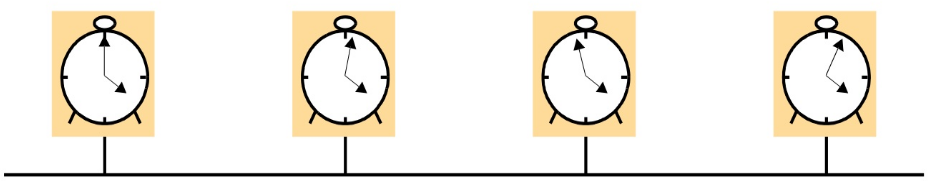
\includegraphics[width=.70\linewidth]{images/Clock/clocks.png}
    \caption{Clock}
\end{figure}

There are N processes \(p_1,p_2,...,p_N\) connected to a network. Each process has a \textbf{local clock}, there is \textbf{no shared memory} and they can communicate only using \textbf{message passing}.

The \textbf{ordering} is defined as follow:
\[e \rightarrow_i e' \quad \textrm{if the event e occurs \textbf{before} e' in process } p_i\]
\[h = <e_i^0,e_1^1,...> \quad \textrm{\textbf{state history of process i}}\]
Where the \textbf{history} represents the sequence of events that take place on the process.

\section{Physical clock}
Synchronization algorithms based on \textbf{physical clocks} operate using local clock of each process.
\[C_i \quad \textrm{we define the local clock of process} p_i \textrm{at physical time t}\]
It is commonly used to consider the timestamp, time indicating when the event occurs.

Two events are successive only if the clock resolution (the time between two successive updates of the clock value) is less than the time interval between the two successive events.

Different local clock can have different values, and it is possible to define:
\begin{itemize}
    \item \textbf{Skew:} difference between two clocks
    \item \textbf{Drift rate:} frequency of the local clock is different from an ideal one
\end{itemize}

A possible idea consists to synchronize local clocks with the \textbf{UTC} (Coordinated Universal Time), which provides the \textbf{real time of the earth}. Synchronization can be:
\begin{itemize}
    \item \textbf{External:} if it is forced by external agents
    \[|S(t) - C_i(t)| < D \quad 1 \leq i \leq N \quad \forall \in I\]
    \begin{itemize}
        \item \(S(t)\) is the real time (provided by UTC)
        \item \(D\) is the precision
        \item \(I\) is the interval of synchronization
    \end{itemize}
    \item \textbf{Internal:} if there is an agreement among a set of processes.
    \[|C_i(t) - C_j(t)| < D \quad 1 \leq i \leq N \quad \forall \in I\]
\end{itemize}

\begin{itemize}
    \item A physical clock H is correct if the drift (difference between the two clock) is within a given threshold \(p > 0\).
    Given \(t, t'\) if \(t' > t\) then
    \[(1 - p)(t' - t) \leq H(t') - H(t) \leq (1 + p)(t' - t)\]
    \item A clock C is defined \textbf{monotone} if it only goes on forward
\end{itemize}

From the physical clock we can define also software clock which is given by:
\[C_i(t) = aH_i(t) + b \quad a, b constants\]

\begin{figure}[!h]
    \centering
    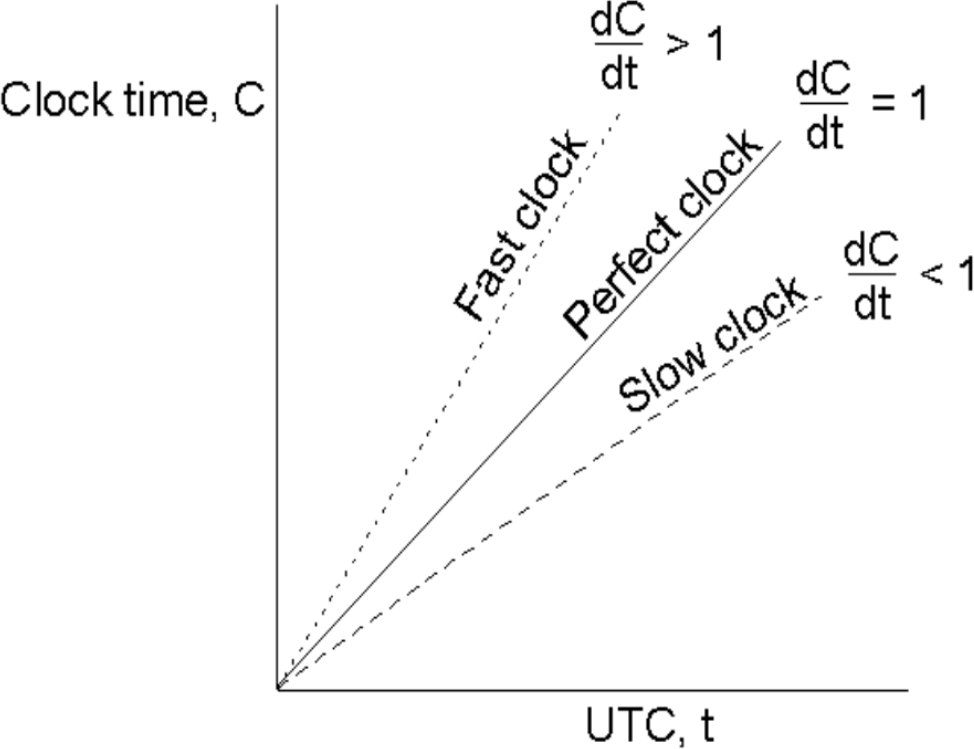
\includegraphics[width=.60\linewidth]{images/Clock/clockDeviance.png}
    \caption{Clock Deviance from real time}
\end{figure}
\newpage

\subsection{Distributed synchronous system}
We begin by considering the simplest possible case: \textbf{synchronization between processes in a synchronous system}. 
One process sends the time t on its local clock to the other in a message m. In principle, the receiving process could set its clock to the time \(t+T_{com}\), where \(T_{com}\) is the time taken to transmit \(m\) between them.

\begin{figure}[!h]
    \centering
    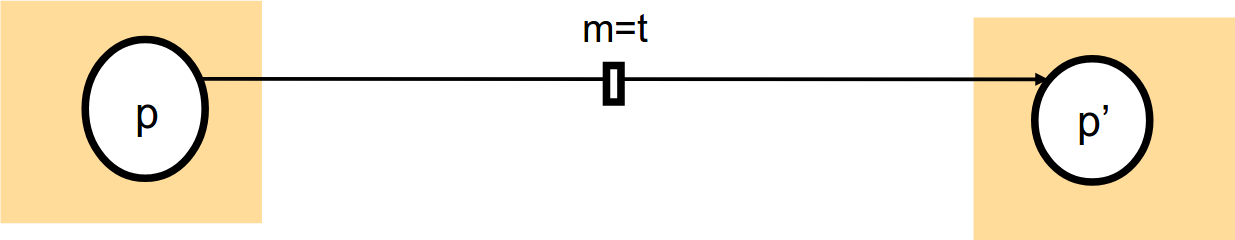
\includegraphics[width=.70\linewidth]{images/Clock/clockSyncInSyncSystem.png}
    \caption{Clock synchronization: Sync. System}
\end{figure}

On this image we have two processes \(p\) and \(p'\) that want to communicate using message passing. \(p\) sends a message with the local clock \(t\) and \(p_0\) receives the message and sets its own local clock to \(t + T_{com}\) (message transmission time).

\begin{itemize}
    \item There is always a minimum transmission time, \(T_{min}\).
    \item In a synchronous system, by definition, there is also an upper bound max \(T_{max}\)
\end{itemize}
From these results some possible choice can be discussed to determine the clock of \(p'\):
\begin{itemize}
    \item If \(p’\) sets the clock to \(t + T_{min} or t + T_{max}\) the error would be \(\leq \delta = (T_{max} - T_{min})\)
    \item If \(p’\) sets the clock to \(t + (T_{min} + T_{max})/2\) the error would be \(\leq \delta/2\)
    \item The optimum bound that can be achieved on clock skew when synchronizing \(N\) clocks is \(\delta(1 - 1/N)\)
\end{itemize}

\subsection{Cristian}
Most distributed systems found in practice are \textbf{asynchronous}: meaning that message delays are not bounded and there is no maximum bound on message transmission delays. For an asynchronous system, we can only say only that \(T_{com} = min + x\) , where \(x > 0\) and it is not known in a particular case. Some algorithms are designed in order to implement clock synchronization for asynchronous systems. The first one was given by Cristian, which suggested the usage of a \textbf{time server}, connected to a device that receives signals from a source of \textbf{UTC}, to synchronize computers externally.

\begin{figure}[!h]
    \centering
    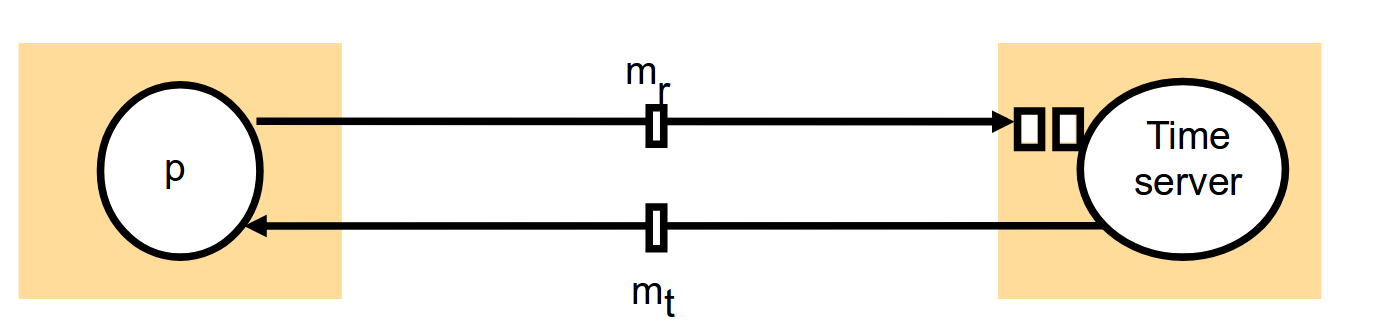
\includegraphics[width=.60\linewidth]{images/Clock/cristianAlg.png}
    \caption{Cristian Algorithm}
\end{figure}

\textbf{Machine point of view:} every machine periodically asks for the time to the time server and when it receives the reply:
\begin{itemize}
    \item It checks the clock
    \item It computes the network delay (at least \(T_{min}\)) as \(T_{round}\), 
    \item It sets the clock to \(t + T_{round}/2\)
\end{itemize}
\textbf{Time server point of view:} when it receives a time request the server puts the
time \(t\) in the reply message just at the last moment useful for sending. The precision \(D\) given by this technique is equal to \(\pm (T_{round} / 2 - T_{min})\)
\begin{itemize}
    \item \textbf{Advantage:} works well when synchronization delay is close to zero
    \item \textbf{Drawbacks:} The usage of a central server reduces and limits reliability and performance
    \item \textbf{Improvements:} using multicast instead of single and central server,, or introduce authentication
\end{itemize}

\subsection{Berkeley}
Berkeley uses a coordinator computer as the master, also called \textbf{active time server}.
\begin{itemize}
    \item Unlike in Cristian’s protocol, this server periodically questions the other computers whose clocks are to be synchronized, called \textbf{slaves}.
    \item The slaves send back their clock values to it.
    \item he master estimates their local clock times by observing the round-trip times (similarly to Cristian’s technique), and it averages the values obtained
\end{itemize}
The master eliminates any occasional readings associated with larger times than this maximum. Instead of sending the updated current time back to the other computers the master sends the amount by which each individual slave’s clock requires adjustment. This can be a positive or negative value.

The Berkeley algorithm eliminates readings from \textbf{faulty clocks}, thus the master takes a \textbf{fault tolerant average.} In other words, the average does not consider the times too far or with abnormal values, meaning that is more \textbf{fault-tolerant} than a simple average.

\subsection{Network Time Protocol (NTP)}
The last two cited algorithm are based on the usage of \textit{centralized system}, now we see an approach based on \textbf{distributed algorithms.}

The \textbf{Network Time Protocol} defines an architecture for a time service and a protocol to distribute time information over the Internet. NTP provides:
\begin{itemize}
    \item Synchronization of the physical clocks respect to UTC
    \item \textbf{Reliable service} that is fault tolerant to connection loss. \textbf{Fault tolerance} is given by redundancy of server and path
    \item \textbf{Scalability} allows frequent synchronization
    \item To provide protection against interference with the time service, whether malicious or accidental
\end{itemize}
The NTP service is provided by a network of servers located across the network.
\begin{itemize}
    \item \textbf{Primary servers} are connected directly to a time source, like UTC
    \item \textbf{Secondary servers} are synchronized with primary servers
    \item The servers are connected in a logical hierarchy called a \textbf{synchronization subnet}, whose levels are called \textbf{strata}
\end{itemize}

\begin{figure}[!h]
    \centering
    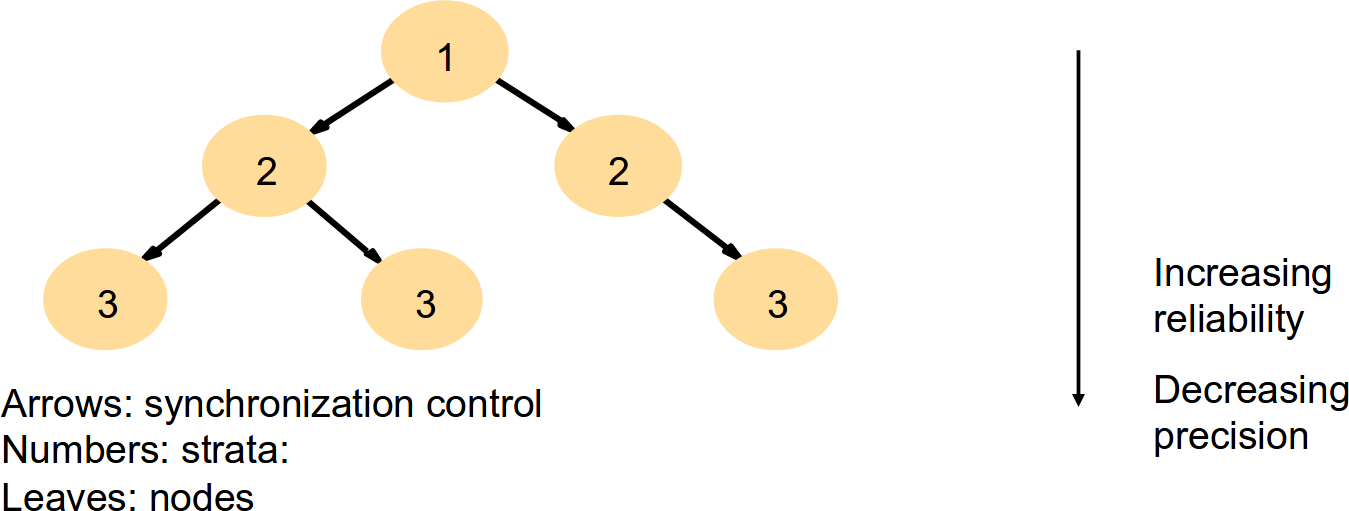
\includegraphics[width=.60\linewidth]{images/Clock/NTP.png}
    \caption{NTP subnet}
\end{figure}

The greater is the number of servers adopted the greater is the reliability provided.
\textbf{Server synchronization} can be done by:
\begin{itemize}
    \item \textbf{Multicast:} common with \textit{high speed LAN}
    \item \textbf{Procedure call:} the server is passive and waits for requests like Cristian's algorithm
    \item \textbf{Symmetrical:} servers exchange messages with timestamp
\end{itemize}

\section{Logical Clock}
In distribute systems since we cannot synchronize clocks perfectly across a distributed system. A different solution is given by \textbf{logical clock}, but first is necessary to give some notions of \textbf{casual ordering.}

\subsection{Casual Ordering}
Consider \(N\) processes, \(p_1,p_2,...,p_N\), we write \(e \rightarrow_i e'\) if event \(e\) \textbf{occurs before} \(e'\) in process \(p_i\). When \(p_i\) sends a message \(m\) to \(p_j\) the event \textit{send(m)} \textbf{precedes} event \textit{receive(m)}:

\[send(m) \rightarrow receive(m)\]

Casual ordering defines order between events and it has some proprieties:
\begin{itemize}
    \item If \(\exists p_i: e \rightarrow_i e'\) then \(e \rightarrow e'\)
    \item \(\forall\) message \(m\) then \(send(m) \rightarrow receive(m)\)
    \item If \(e, e', e''\) are events:
    \[e \rightarrow e', e' \rightarrow e'' \quad e \rightarrow e''\]
    \item Even \(a\) and \(b\) can be \textbf{concurrent} and we denote this propriety as \(a||b\). Meaning that they are \textbf{not related} 
\end{itemize}

\begin{figure}[!h]
    \centering
    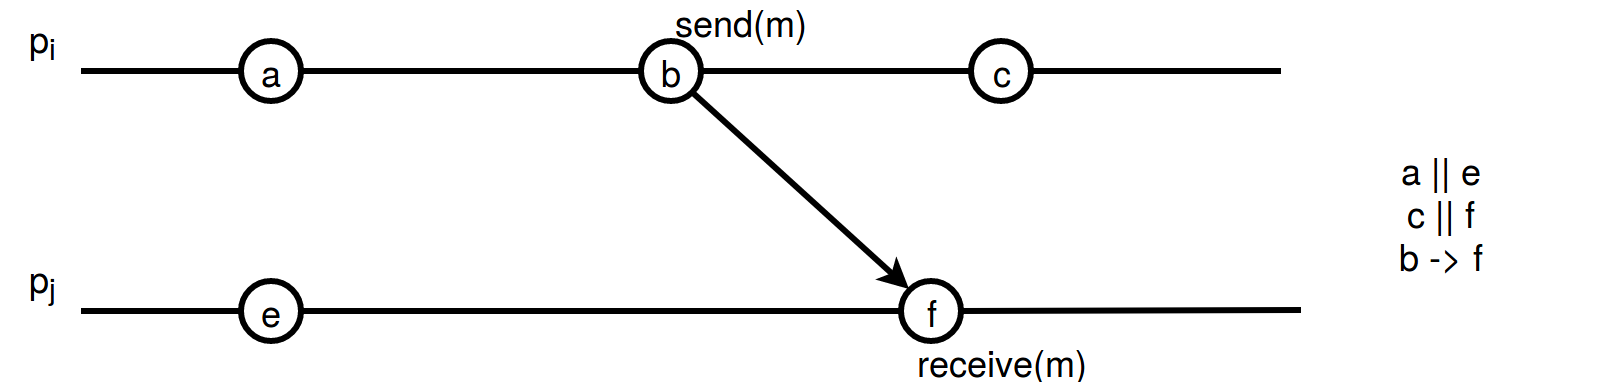
\includegraphics[width=.60\linewidth]{images/Clock/causalOrdering.png}
    \caption{Casual Ordering Example}
\end{figure}

\subsection{Lamport timestamp}
It is independent from physical clock and it is basically a software counter. Each process \(p_i\) keeps its own \textbf{logical clock}, \(L_i\), which it uses to apply the so called \textbf{Lamport timestamp} to events. Moreover we denote the \textbf{timestamp} of event \(e\) at \(p_i\) by \(L_i(e)\)
Processes update their logical clocks and transmit the values of their logical clocks in messages as follows:
\begin{itemize}
    \item \textbf{LC1:} \(L_i\) is incremented before each event is managed at process \(p_i\).
    \item \textbf{LC2:} If \(p_i\) sends a message \(m\) it sends in \textbf{piggybacking} the value \(t = L_i\). If \(p_j\) receives a message (m,t) it sets \(L_j = max(L_j,t)\) and applies \textbf{LC1} for the event \textit{receive(m)}.
\end{itemize}

\begin{figure}[!h]
    \centering
    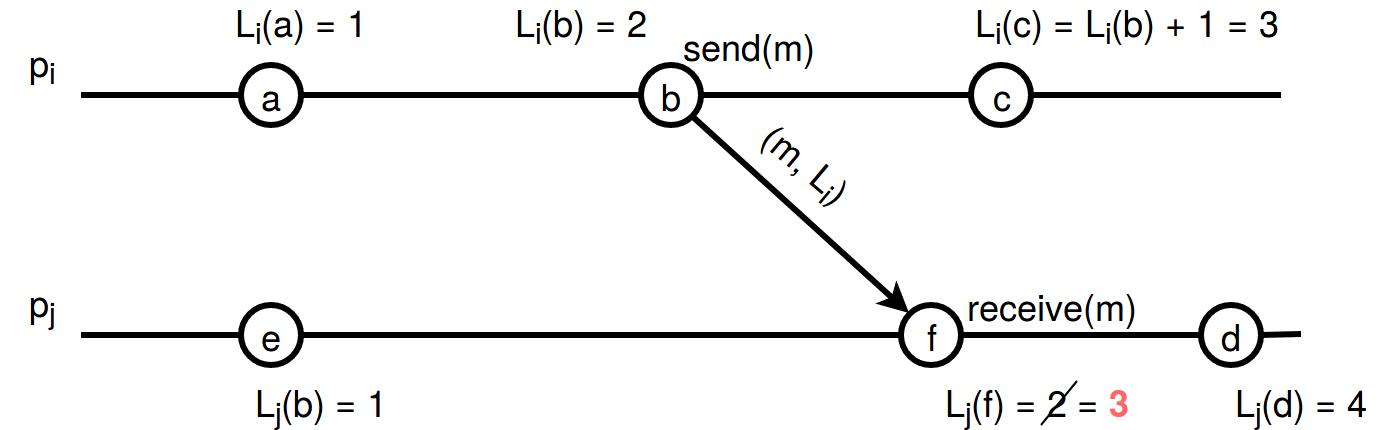
\includegraphics[width=.60\linewidth]{images/Clock/logicalClock.png}
    \caption{Logical clock algorithm example}
\end{figure}
\newpage

Logical clock has the monotonicity property, meaning that:
\[\textrm{If} e \rightarrow e' \quad \textrm{then} \quad L(e)<L(e')\]

\subsection{Vector clock}
\begin{itemize}
    \item Some pairs of distinct events, generated by different processes, have numerically identical Lamport timestamps
    \item However, we can create a global ordering of events by taking into account the pair (timestamp,\(p_i\)).
\end{itemize}
If \(e\) is an \textbf{event occurring} at \(p_i\) with \textbf{local timestamp} \(T_i\), and \(e'\) is an \textbf{event occurring} at \(p_j\) with \textbf{local timestamp} \(T_j\), we define the \textbf{global logical timestamps} for these events to be: \(T_i, i\) and \(T_j, j\) respectively. And we define

\[(T_i, i) < (T_j, j) \iff T_i < T_j \vee (T_i = T_j \wedge i < j)\]

A different ordering that overcomes the iff limitation of the Lamport definition, \(L(e) < L(e') \textrm{not} e<e'\), is the \textbf{vector clock}. To each process \(p_i\) we associate a \textbf{vector of clocks \(V_i\)} used for local timestamp.

\begin{figure}[!h]
    \centering
    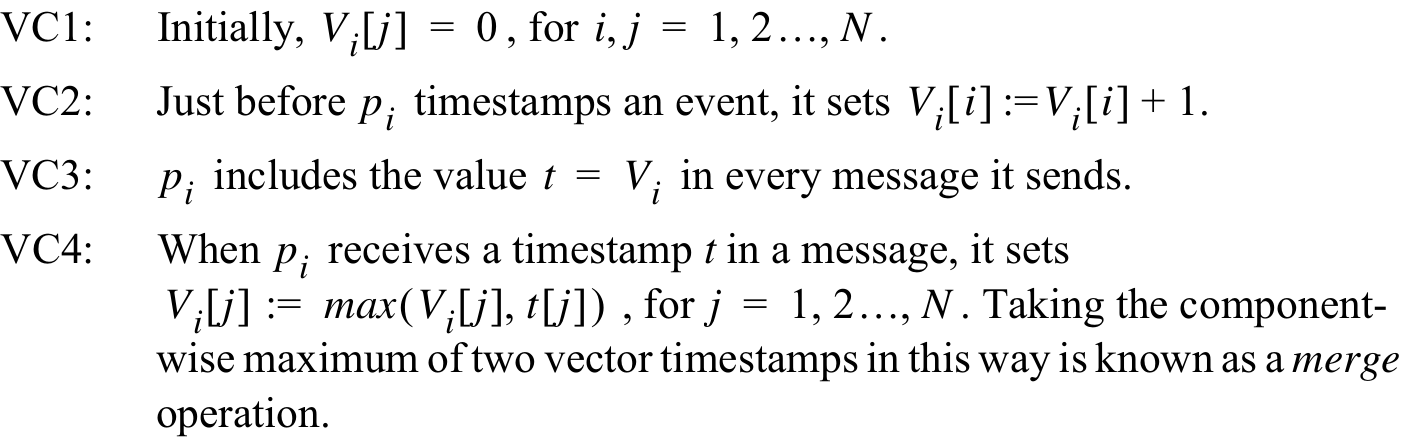
\includegraphics[width=.90\linewidth]{images/Clock/vectorClockAlg.png}
    \caption{Vector Clock Algorithm}
\end{figure}

\begin{itemize}
    \item \(V_i[i]\) represent the event number occurred in \(p_i\) and marked by \(p_i\)
    \item \(V_i[j]\) represent the event number occurred in \(p_j\) and potentially affected \(p_i\)
\end{itemize}
Then:
\[V(e) < V(e') \quad e < e'\]
\[V = V' \iff V[i] = V'[i] \quad \forall i = 1,..,N\]
\[V \leq V' \iff V[i] \leq V'[i] \quad \forall i = 1,..,N\]
\[V < V' \iff V[i] \leq V'[i] \wedge V \neq V' \quad \forall i = 1,..,N\]
 \newpage
\begin{figure}[!h]
    \centering
    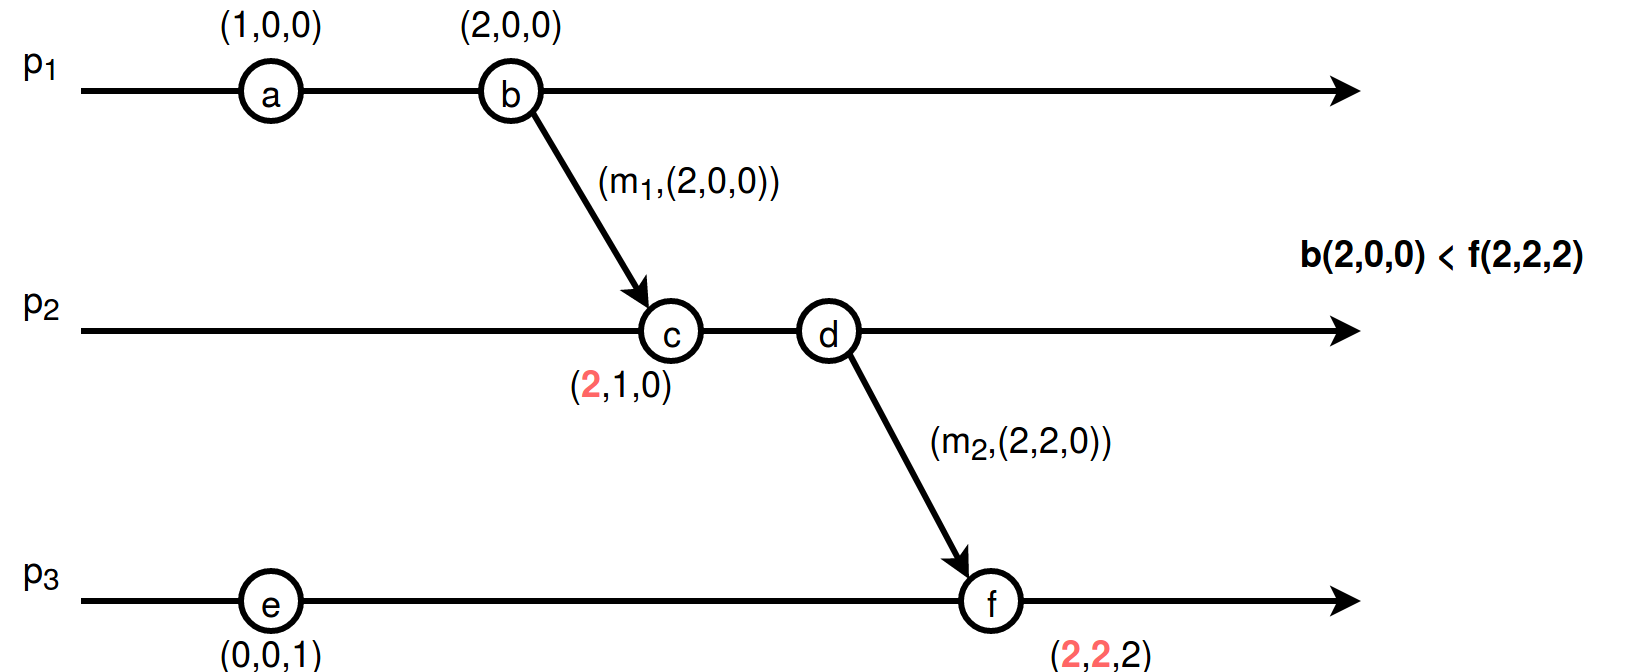
\includegraphics[width=.60\linewidth]{images/Clock/vectorClock.png}
    \caption{Vector Clock algorithm example}
\end{figure}

The main drawback of this strategy is that it requires memory space to store the vector \(V\) and message dimension increase proportional to \(N\).

\section{Global state}
Another fundamental problem consists to \textbf{verify global properties in a distributed system.} We begin by giving the examples of a distribute system in which deadlock between two or more processes can happen.

\begin{figure}[!h]
    \centering
    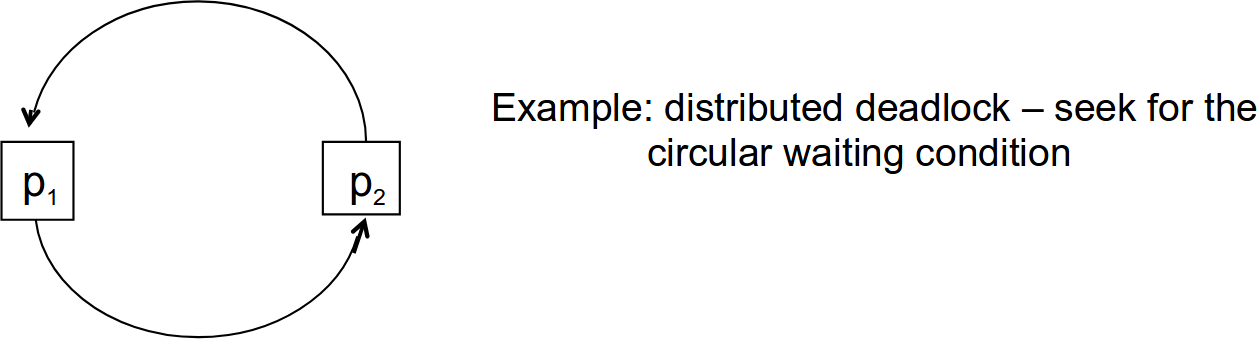
\includegraphics[width=.60\linewidth]{images/Clock/deadlockGlobalProp.png}
    \caption{Global state deadlock}
\end{figure}

As it is possible to see is fundamental to study properties of the system for \textbf{know better what it can happen and possible issues}. Knowing the \textbf{global state of the system} sometimes can solve some problems.
The essential problem is the absence of global time. If all processes had perfectly synchronized clocks, then we could agree on a time at which each process would record its state. From the collection of process states we could tell, for example, whether the processes were deadlocked. But we cannot achieve perfect clock synchronization, so this method is not available to us.

Each process \(p_i\) is associated to a local state history: \(h_i = <e_i^0, e_i^1,...>\)
\begin{itemize}
    \item \(e_i^k\) k-th event in the local history of \(p_i\). Local state history of process \(p_i\) up to \(k\) is so defined:  \(h_i = <e_i^0, e_i^1,.... e_i^k>\)
    \item \(s_i^k\) state of \(p_i\) just after occurrence of event \(e_i^k\)
    \item \(s_i^0\) initial state of \(p_i\)
\end{itemize}

Global state history of set of processes \(\{p_1,p_2,...,p_N\}\)
\[H = \bigcup_{i=1}^{N}h_i\]
\[S = \{s_1,s_2,..,s_N\} \quad \textrm{\textbf{global state}}\]

But now the question is spontaneous: \textbf{Which are the significant states?}

\textbf{Distributed snapshot} is an algorithm used to derivate a global state in which the distributed system can be. It defines a consistent \textbf{global state}.

\[C = \bigcup_{i=1}^{N}h_i^{c_i} \quad C \rightarrow \{e_1^{c_1},...,e_N^{c_N}\}\]

\subsection{Consistent global state}
A cut of a distributed system is said to be \textbf{consistent} if for each event included in the cut, it also includes the related events according to \textit{happened-before}:
\[\forall e \in C \quad e' \rightarrow e \quad \rightarrow \quad e' \in C\]

\begin{figure}[!h]
    \centering
    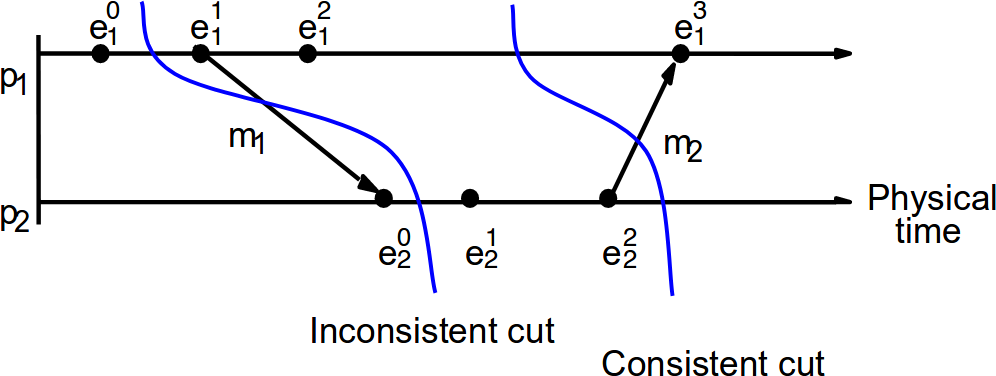
\includegraphics[width=.60\linewidth]{images/Clock/consistentState.png}
    \caption{Consistent and Inconsistent state}
\end{figure}

A \textbf{global state is said to be consistent if it corresponds to a consistent cut.} A global execution is a succession of global consistent states \(S_0 \rightarrow S_1 \rightarrow S_2 \rightarrow ....\) A \textbf{consistent run} is an ordering of the events in a global history that is consistent with this happened-before relation \(o \rightarrow \textrm{on} H\).

\subsection{Distributed snapshot}
Chandy and Lamport describe a \textbf{snapshot algorithm} for determining global states of distributed systems, which we now present. The \textbf{goal} of the algorithm is to \textbf{record a set of process and channel states} (a snapshot) for a set of processes \(p_i (i = 1, 2, ..., N)\).  The algorithm records state locally at processes. An obvious method for gathering the state is for all processes to send the state they recorded to a designated collector process.

The algorithm assumes that:
\begin{itemize}
    \item Reliable channel and communication.
    \item Channel is unidirectional and provide FCFS-ordered message delivery.
    \item The graph of processes and channels is strongly connected
    \item Any process may initiate a global snapshot at any time
    \item The processes may continue their execution and send and receive normal messages while the snapshot takes place.
\end{itemize}
A process that starts records its own state and then sends a special message (\textbf{marker}) on all the outgoing channels to other processes to gather the global state. 